
% !TeX spellcheck = en

\chapter{Database Change Scenarios}
This section shows how to handle the predefined scenarios for the given change management tool. This includes following scenarios: 

\begin{itemize}
	\item Rename an attribute.
	\item Add an attribute and set the value as a constant.
	\item Delete an attribute.
	\item Change an attribute type and add an SQL script to fill it from existing values.
	\item Rename a table and change a related view which uses this table.
	\item Split a column into two columns
\end{itemize}

The changes were applied to an existing database Pagila \cite{Hillyer}. Each first two migrations are to setup the database, first the create the schema and second to insert the specific data.

\section{Flyway Scenarios}

\subsection{Using CLI}
\marginpar{Setup \cite{FlywayGetStarted}}%
To create a first migration, add a database change as sql file into the sql directory (see \autoref{fig:flyway_folder_structure}). 
The scripts \texttt{V1\_\_create\_db.sql} and \texttt{V2\_\_insert\_pagila\_data.sql} set up the pagila database as illustrated in \autoref{fig:flyway_empty_db}. When running  \texttt{flyway migrate}, flyway wants to adapt the schema history table. But as this table does not exist, it will create a new one instead.


 

\begin{figure}[H]
	\centering
	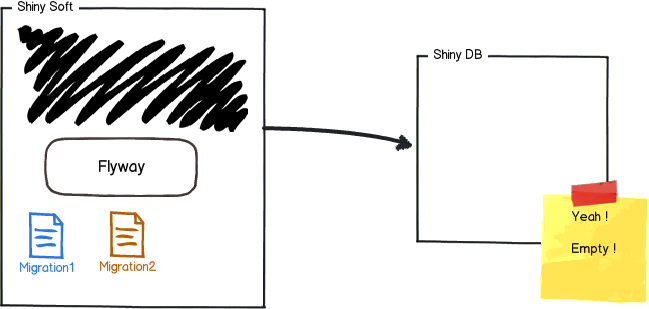
\includegraphics[width=0.45\textwidth]{./chapters/scenarios/images/EmptyDb}
	\caption[Flyway empty database - Source: \cite{FlywayGetStarted}]{Flyway empty database}
	 \label{fig:flyway_empty_db}
\end{figure}
Now the table \textit{flyway\_schema\_history} has been created via the first flyway migration. This metadata table holds various information regarding the database migrations and their history. After this initialization, flyway runs the migration scripts in the sql directory according on their version number subsequently. 
BASELINE MODEL! To start with a baseline

\begin{figure}[H]
	\centering
	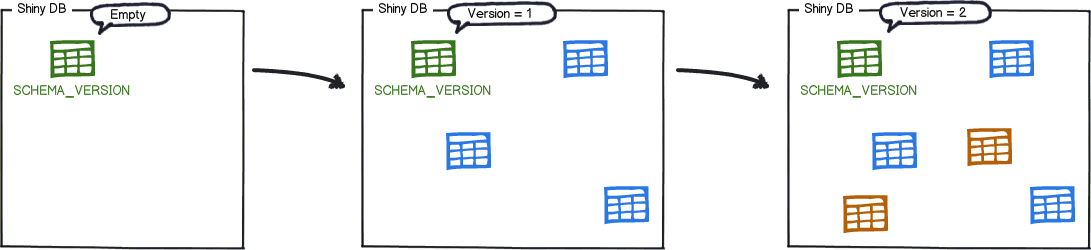
\includegraphics[width=0.85\textwidth]{./chapters/scenarios/images/Migration-1-2}
	\caption[Flyway first migrations - Source: \cite{FlywayGetStarted}]{Flyway first migrations}
	\label{fig:Migration-1-2}
\end{figure}


\marginpar{Rename an attribute}%
The first change specific migration is in the sql migration script\\ \texttt{V3\_\_rename\_attribute.sql}:
\begin{lstlisting}[language=SQL]
ALTER TABLE customer RENAME COLUMN email TO private_email;
\end{lstlisting}
After just adding the script to de sql directory, flyway already knows the change and stores it into the meta data table. With \texttt{flyway info} the migration status can be asked:

\begin{figure}[H]
	\centering
	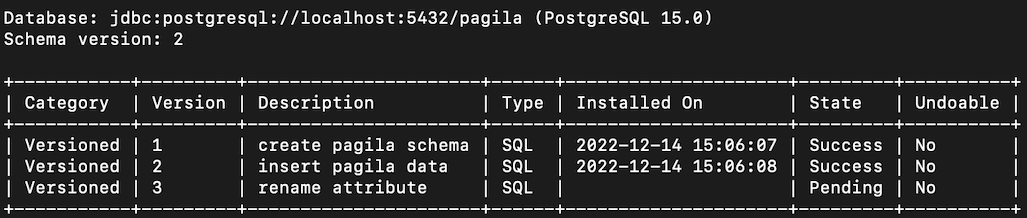
\includegraphics[width=0.95\textwidth]{./chapters/scenarios/images/flyway_metadata_v2}
	\caption[Flyway meta data table - Source: Own illustration]{Flyway meta data table}
	% \label{fig:bsp_chapter:example_figure}
\end{figure}
In order to perform the migration effectively, the command \texttt{flyway migrate} is applied.



\marginpar{Add an\\ attribute}%
To apply the second migration the following script is applied in V3.
\begin{lstlisting}[language=SQL]
ALTER TABLE customer ADD COLUMN gender VARCHAR(50);

UPDATE customer
SET gender = 'undefined';
\end{lstlisting}
Flyway generates a checksum for every applied migration. This checksum is used to track if a file was changes after its applied migration. If such a change occurs, a new migration will cause an error and asks to either revert the change or to run \texttt{flyway repair} to update the schema history.
If a developer would change the default value of gender from \textit{undefined} to \textit{undef} and run a new migration, it would fail. To fix this run \texttt{flyway repair}. Even the environment is now fixed, the change gender equals \textit{undef} is not applied and still \textit{undefined}.


\marginpar{Delete an\\ attribute}%

\begin{lstlisting}[language=SQL]
ALTER TABLE customer
DROP COLUMN gender;
\end{lstlisting}


\marginpar{Change an attribute typ}%
To change an attribute type the migration in the file \texttt{V6\_\_change\_attribute\_type.sql} was applied with flyway migrate:
\begin{lstlisting}[language=SQL]
ALTER TABLE customer
ALTER COLUMN private_email TYPE VARCHAR(100) USING private_email::varchar;
\end{lstlisting}


\marginpar{Rename a table and change related view}%
The next migration is to change a related view after renaming a table\\
\texttt{V7\_\_change\_attribute\_type.sql} was applied with flyway migrate:
\begin{lstlisting}[language=SQL]
ALTER TABLE customer RENAME TO clients;
	
	
CREATE OR REPLACE VIEW customer_list AS
SELECT cl.customer_id AS id,
	(cl.first_name || ' '::text) || cl.last_name AS name,
	a.address,
	a.postal_code AS "zip code",
	a.phone,
	city.city,
	country.country,
	CASE
		WHEN cl.activebool THEN 'active'::text
		ELSE ''::text
	END AS notes,
	cl.store_id AS sid
FROM clients cl
JOIN address a ON cl.address_id = a.address_id
JOIN city ON a.city_id = city.city_id
JOIN country ON city.country_id = country.country_id;
\end{lstlisting}

After this second to last migration the flyway schema history looks like the following:
\begin{figure}[H]
	\centering
	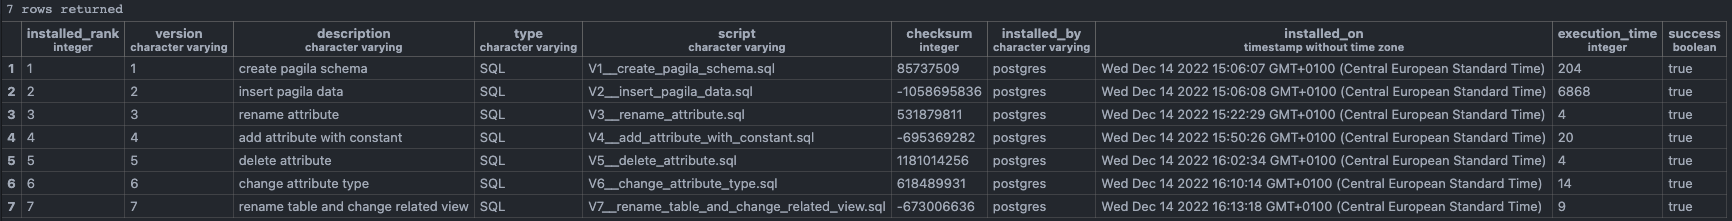
\includegraphics[width=1.1\textwidth]{./chapters/scenarios/images/flyway_schema_history}
	\caption[Flyway Schema History - Source: Own illustration]{Flyway Schema History}
	% \label{fig:bsp_chapter:example_figure}
\end{figure}
For every migration the date inclusive time, the script or the user that applied the script is stored.

\newpage
\marginpar{Split a column}%
First two new columns are created and then the string is split and distributed into the two new columns.

\begin{lstlisting}[language=SQL]
ALTER TABLE address ADD COLUMN street text;
ALTER TABLE address ADD COLUMN house_number text;


WITH results AS (
	SELECT address_id as id,
	(string_to_array(address, ' '))[1] as a1,
	array_to_string((string_to_array(address, ' '))[2:], ' ') as a2
	from address
)

UPDATE address
SET house_number = (SELECT a1 FROM results WHERE address_id = results.id),
street = (SELECT a2 FROM results WHERE address_id = results.id);
\end{lstlisting}

All migrations could be implemented in PostgreSQL and executed without any problems. There were no limitations or problems with any of the migrations.


\marginpar{Failed\\ migration \cite{Lukonin2017}}%
Flyway automatically wraps every migration script in a transaction, which allows for automatic rollback in case of an error. If your database supports DDL transactions (such as PostgreSQL), the entire migration script will be rolled back automatically. However, if you are using SQL Server, the DDL queries will be committed automatically, so you will need to create manual rollback scripts or use idempotent scripts to roll back the changes. If your migration script does not contain DDL commands, it will generally be automatically rolled back by most database engines in case of an error.\\
To make the rollback process easier, Flyway supports rollback scripts, which can be created for every versioned migration file using the naming convention \textit{U\#\#\#\_\_text.sql}. If a migration fails, Flyway will automatically run the corresponding rollback script. The UNDO command (see \autoref{flyway_features}) can also be used to manually trigger a rollback, which will roll back the latest migration by default. Alternatively, taking a snapshot of the database before release and restoring it if any migration goes wrong is the cleanest approach, but may not always be feasible. It is important to have a well-designed rollback strategy in place, which may involve creating proper rollback scripts and using idempotent migrations to make the process easier.

\newpage
\subsection{Usage with Java API}
\marginpar{Java Migration}%
Flyway is most useful when integrated into an application. By doing so, the compatibility between the application and its database can be maintained automatically, without the need for manual intervention. Flyway checks the version of the database and automatically applies new migrations before the rest of the application begins. This is crucial because the database must be in a state that is compatible with the rest of the code before the application can function properly. Hereby flyway can use migration files written in classic SQL in the directory \textit{src/main/resources/db.migration/}, similar to the last chapter.

\begin{lstlisting}[language=Java]
import org.flywaydb.core.Flyway;

public class App {
	public static void main(String[] args) {
		// Create the Flyway instance and point it to the database
		Flyway flyway = Flyway.configure().dataSource("jdbc:h2:file:./target/foobar", "sa", null).load();
		flyway.migrate(); // Start the migration
	}
}
\end{lstlisting}

\marginpar{Java Migration}%
Another option is to implement the migrations directly as a Java class. Running Flyway through the API on application startup is the most efficient and reliable method. This method allows you to combine all migrations with your application, making it easy to deploy to any environment. The API will automatically detect the state of the database and perform the necessary migrations on startup, ensuring that your application code is always compatible with the database it is accessing.
Flyway can be integrated in Gradle or Maven as in the following example.

%\begin{lstlisting}[language=Java, caption={File: src/main/java/db/migration/V1\_\_create_\pagila\_schema.sql}]
\begin{lstlisting}[language=Java, caption={File: src/main/java/db/migration/V3\_\_rename\_attribute.sql}]
package db.migration;

import org.flywaydb.core.api.migration.BaseJavaMigration;
import org.flywaydb.core.api.migration.Context;
import java.sql.PreparedStatement;

public class V1__RenameAttribute extends BaseJavaMigration {
	public void migrate(Context context) throws Exception {
		try {
			PreparedStatement statement = context.getConnection().prepareStatement("ALTER TABLE customer RENAME COLUMN email TO private_email;")) {
						statement.execute();
			}
	}
}
\end{lstlisting}

With the command below the migration can be applied.
 \begin{lstlisting}
mvn flyway:migrate
 \end{lstlisting}


\newpage
\section{Liquibase Scenarios}
\subsection{SQL-Changelog}
\marginpar{SQL-Changelog}%

\subsection{YAML-Changelog}
\marginpar{YAML-Changelog}%


\newpage